\documentclass[tikz,border=3pt]{standalone}
\usepackage[utf8]{inputenc}
\usepackage[T1]{fontenc}
\usepackage{lmodern}
\renewcommand{\familydefault}{\sfdefault}
\usepackage{sansmath}\sansmath
\usepackage{chemfig}
\usepackage{pgfplots}\pgfplotsset{compat=1.18,/pgf/number format/use comma,/pgf/number format/1000 sep={.}}
\usetikzlibrary{arrows.meta,calc,positioning,decorations.pathmorphing,patterns}
% paleta del sitio
\definecolor{nar}{HTML}{E8680C}\definecolor{narc}{HTML}{FFB35C}\definecolor{hielo}{HTML}{FFF3E8}
\definecolor{tinta}{HTML}{1D1D1F}\definecolor{gris}{HTML}{6E6E73}\definecolor{lila}{HTML}{7C5CF0}
\definecolor{azul}{HTML}{2F6FD6}\definecolor{menta}{HTML}{17A673}\definecolor{coral}{HTML}{E8342A}
\begin{document}
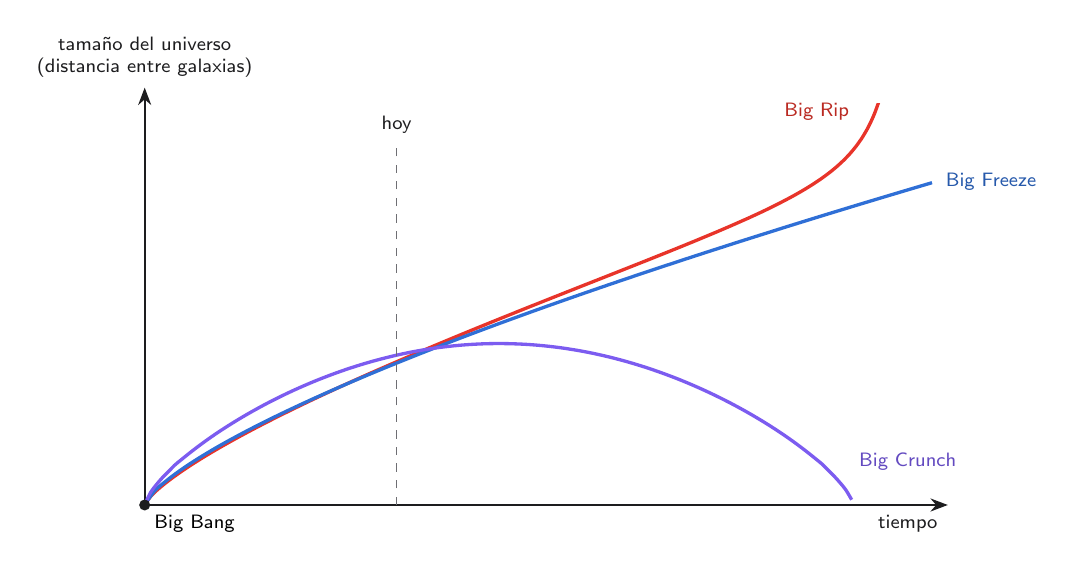
\begin{tikzpicture}[font=\footnotesize,>={Stealth[length=2.2mm]}]
\draw[->,thick,tinta] (0,0) -- (10.2,0) node[below left,font=\scriptsize] {tiempo};
\draw[->,thick,tinta] (0,0) -- (0,5.3) node[above,font=\scriptsize,align=center] {tamaño del universo\\(distancia entre galaxias)};
\begin{scope}
\clip (0,0) rectangle (10,5.1);
\draw[coral,very thick,domain=0.001:9.6,samples=120,smooth] plot (\x,{0.75*\x^0.75 + 0.5/(9.75-\x) - 0.5/9.75});
\end{scope}
\draw[azul,very thick,domain=0.001:10,samples=80,smooth] plot (\x,{0.78*\x^0.72});
\draw[lila,very thick,domain=0.001:8.98,samples=120,smooth] plot (\x,{2.05*(sin(180*\x/9))^0.7});
\fill[tinta] (0,0) circle (0.07); \node[below right,font=\scriptsize] at (0,0) {Big Bang};
\draw[gris,dashed] (3.2,0) -- (3.2,4.6) node[above,font=\scriptsize,text=tinta] {hoy};
\node[anchor=west,font=\scriptsize,text=coral!80!black] at (8.0,5.0) {Big Rip};
\node[anchor=west,font=\scriptsize,text=azul!80!black] at (10.05,4.1) {Big Freeze};
\node[font=\scriptsize,text=lila!80!black,anchor=west] at (8.95,0.55) {Big Crunch};
\end{tikzpicture}
\end{document}
